\documentclass[12pt]{extarticle}
\usepackage{amsmath, amsthm, latexsym, tikz, graphicx, listings, microtype, mathtools, soul, color, fancyhdr}
\usepackage[margin=1in]{geometry}

\newenvironment{myindentpar}[1]%
 {\begin{list}{}%
         {\setlength{\leftmargin}{#1}}%
         \item[]%
 }
 {\end{list}}
 
\DeclarePairedDelimiter\abs{\lvert}{\rvert}%
\DeclarePairedDelimiter\norm{\lVert}{\rVert}%

% Swap the definition of \abs* and \norm*, so that \abs
% and \norm resizes the size of the brackets, and the 
% starred version does not.
\makeatletter
\let\oldabs\abs
\def\abs{\@ifstar{\oldabs}{\oldabs*}}
%
\let\oldnorm\norm
\def\norm{\@ifstar{\oldnorm}{\oldnorm*}}
\makeatother

\definecolor{lightgray}{gray}{0.65}
\definecolor{pinegreen}{RGB}{1, 171, 161}
\definecolor{lightblue}{RGB}{135, 206, 250}
\definecolor{dkgreen}{rgb}{0,0.6,0}
\definecolor{gray}{rgb}{0.5,0.5,0.5}
\definecolor{mauve}{rgb}{0.58,0,0.82}
\definecolor{darkblue}{rgb}{0.0,0.0,0.6}
\definecolor{cyan}{rgb}{0.0,0.6,0.6}

\newcommand*{\Value}{\frac{1}{2}x^2}%
\newcommand{\hlc}[2][yellow]{ {\sethlcolor{#1} \hl{#2}} }

\definecolor{codegray}{gray}{0.9}
\newcommand{\code}[1]{\colorbox{codegray}{\texttt{#1}}}

% /*--------------------------------------------------------------*/
%   Changing the values here sets the due date for the assignment!
% /*--------------------------------------------------------------*/
\newcommand{\duedate}{XX/XX/XX }
\newcommand{\semester}{SEMESTER}

\lstset{frame=tb,
  language=C++,
  breaklines=true,
  showstringspaces=false,
  columns=flexible,
  numbers=none,
  tabsize=3,
  escapeinside={(*@}{@*)}
  %,
  %commentstyle=\color{dkgreen},
  %stringstyle=\color{mauve}
}
\pagestyle{fancy}
\fancyhf{}
\renewcommand{\headrulewidth}{0pt}
\lhead{\color{lightgray} CSCE-313}
\rhead{\color{lightgray} \semester}
\rfoot{\thepage}
\pagenumbering{arabic}

\begin{document}

\begin{center}
    \underline{{\large Machine Problem 4: UNIX Processes \  }(Due: \duedate)}  \\
\end{center}


\ \\
{\large \underline{Introduction}:}

\ \\
The /proc directory is a pseudo filesystem that allows access to kernel data structures while in user space. It allows you to view some of the information the kernel keeps on running processes. To view information about a specific process you just need to view files inside of the directory: /proc/[pid]. For more information simply view the manpage with man proc.  

\ \\
{\large \textbf{The Assignment}:} \newline
\ \\
Using the files stored at /proc write a program/script to find information about a specific process using a user provided pid. In the following, you will find a list of the task\_struct members for which you are required to find their value. In the task\_struct a lot of the data you are finding is not represented as member values but instead pointers to other linux data structures that contain these members. All of the information you will be retrieving can be found in a process’s proc directory (/proc/[pid]).  Your program must be able to retrieve the following data about any given process:  


\begin{center}
    \textbf{Table \#1: Process Attributes}
\end{center}
\begin{displaymath}
    \begin{array}{|l|l|l|}
    \hline
    \text{Category} & \text{Required Variables/Items} & \text{Description} \\ 
    \hline
        \text{Identifiers} & \text{PID, PPID}    & \text{Process ID of the current process and its parent} \\
        \hspace{1cm}       & \text{EUID, EGID}   & \text{Effective user and group ID} \\
        \hspace{1cm}       & \text{RUID, RGID}   & \text{Real user and group ID} \\
        \hspace{1cm}       & \text{FSUID, FSGID} & \text{File system user and group ID} \\
    \hline
        \text{State}       & \text{R, S, D, T, Z, X} & \text{Running, Sleeping, Disk sleeping, Stopped,} \\ \hspace{1cm}       & \hspace{1cm}            & \text{Zombie, and Dead} \\
    \hline
        \text{Thread }     & \text{Thread\_Info} & \text{Thread IDs of a process} \\
        \text{Information} & \hspace{1cm}        & \hspace{1cm}\\
    \hline
        \text{Priority}    & \text{Priority Number} & \text{Integer value from 1 to 99} \\
        \hspace{1cm}       & \text{Niceness Value}  & \text{Integer value from -20 to 19} \\
    \hline
        \text{Time}        & \text{stime \& utime}  & \text{Time that a process has been scheduled} \\
        \text{Information} & \hspace{1cm}           & \text{in kernel/user mode} \\
        \hspace{1cm}       & \text{cstime \& cutime} & \text{Time that a process has waited on children}\\
        \hspace{1cm}       & \hspace{1cm}            & \text{being run in kernel/user mode} \\
    \hline
        \text{Address} & \text{Startcode \& Endcode} & \text{The start and end of a process} \\
        \text{Space}   & \text{ESP \& EIP}           & \text{in memory} \\
    \hline
        \text{Resources} & \text{File Handles \&} & \text{Number of fds used, and number of} \\
        \hspace{1cm}     & \text{Context Switches} & \text{voluntary/involuntary context switches} \\
    \hline
        \text{Processors} & \text{Allowed processors and} & \text{Which cores the process is allowed to run on,} \\
        \hspace{1cm}      & \text{Last used one} & \text{and which one was last used} \\
    \hline
        \text{Memory} & \text{Address range, permissions} & \text{Output a file containing the process's} \\
        \text{Map}    & \text{offset, dev, inode,} & \text{currently mappped memory regions} \\
        \hspace{1cm}  & \text{and path name}       & \hspace{1cm} \\
    \hline
    \end{array}
\end{displaymath}

\ \\
{\large \underline{Deliverables}:}
\begin{itemize}
    
    \item \textbf{Code}: 
    \begin{itemize}
    
        \item You are to turn in one file ZIP file, named $<$Last Name$>$\_$<$First Name$>$\_MP3.zip, which contains your program/script named proctest.cpp/proctest.py/proctest.sh (c++, python, and bash names respectively).  If your implementation consists of more than one file, include those and a makefile (if applicable).  
    
    \end{itemize}
    \item \textbf{Report}:
    \begin{itemize}
    
        \item Answer the following additional questions
        \begin{enumerate}
        
            \item For a process run by a user other than yourself, find the following items from Table \#1: [Identifiers, State, Thread Information, Priority, Time Information, Resources, and Memory Map]
            \item For a process that you have created, retrieve all items enumerated in Table \#1.  
            \item What are the differences between the real and effective IDs, and what is a situation where these will be different?
            \item Why are most of the files in /proc read only?
            \item Why is the task\_struct so important to the kernel and what is it used for?
        
        \end{enumerate}
    
    \end{itemize}
    
\end{itemize}


\ \\
{\large \underline{Advanced Concepts}:}

\begin{myindentpar}{5mm}

    \ \\
    \textbf{Task\_Struct Members}
    
    \ \\
    Linux and UNIX distributions organize all internal process data into structures named task\_struct.  The kernel maintains one task\_struct member for each process running on the system.  Each task\_struct member contains two pointers specifically designated to point to other task\_struct members.  As such, the kernel organizes all task\_struct members into linked lists.  On startup, the kernel also initializes a pid hash table whose elements are linked lists.  This is done to save some time searching for process data structures.  Instead of having to search one large list (for perspective, pid\_max on the author's Debian 8 system is $2^{15}$), the kernel quickly hashes the process pid into one of the hash table elements and then searches a much smaller list to find the correct task\_struct member (Bovet, 81 \& Glass, 555).    
    
    \ \\
    A visual description of the organization of the task\_struct structure is provided in Figure 1.  Also provided, for the curious reader, is the entire listing of all task\_struct members.  Inside, you should be able to see all of the fields that you are required to find for the assignment (or at least pointers to other kernel data structures that actually contain those fields).  For even further reading see \textit{Bovet} and \textit{Glass} in the bibliography section

    \begin{center}
        Figure \#1: Task Struct Members \& Fields (Glass, 554)
    \end{center}
    \begin{center}
        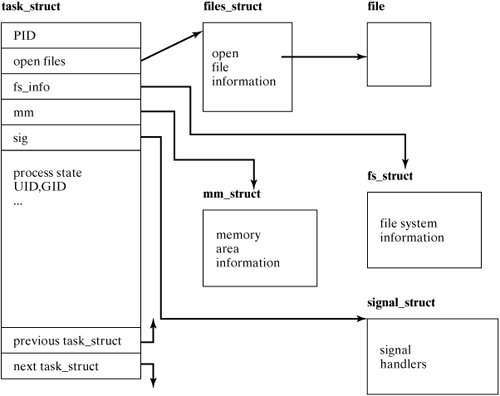
\includegraphics{task_struct.png}
    \end{center}
    
    \vspace{10mm}
    \begin{center}
        Figure \#2: Pid Hash Table (Glass, 555)
    \end{center}
    \begin{center}
        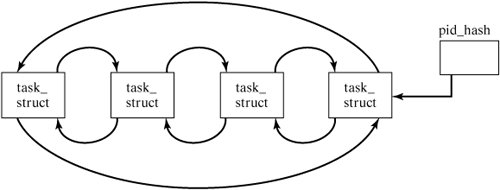
\includegraphics{pid_hash.png}
    \end{center}

\newpage
\begin{center}
    Example \#1: task\_struct Declaration
\end{center}
\begin{lstlisting}[frame=single]
struct task_struct {
/* these are hardcoded - don't touch */
  volatile long        state;          /* -1 unrunnable, 0 runnable, >0 stopped */
  long                 counter;
  long                 priority;
  unsigned             long signal;
  unsigned             long blocked;   /* bitmap of masked signals */
  unsigned             long flags;     /* per process flags, defined below */
  int errno;
  long                 debugreg[8];    /* Hardware debugging registers */
  struct exec_domain   *exec_domain;
/* various fields */
  struct linux_binfmt  *binfmt;
  struct task_struct   *next_task, *prev_task;
  struct task_struct   *next_run,  *prev_run;
  unsigned long        saved_kernel_stack;
  unsigned long        kernel_stack_page;
  int                  exit_code, exit_signal;
  /* ??? */
  unsigned long        personality;
  int                  dumpable:1;
  int                  did_exec:1;
  int                  pid;
  int                  pgrp;
  int                  tty_old_pgrp;
  int                  session;
  /* boolean value for session group leader */
  int                  leader;
  int                  groups[NGROUPS];
  /* 
   * pointers to (original) parent process, youngest child, younger sibling,
   * older sibling, respectively.  (p->father can be replaced with 
   * p->p_pptr->pid)
   */
  struct task_struct   *p_opptr, *p_pptr, *p_cptr, 
                       *p_ysptr, *p_osptr;
  struct wait_queue    *wait_chldexit;  
  unsigned short       uid,euid,suid,fsuid;
  unsigned short       gid,egid,sgid,fsgid;
  unsigned long        timeout, policy, rt_priority;
  unsigned long        it_real_value, it_prof_value, it_virt_value;
  unsigned long        it_real_incr, it_prof_incr, it_virt_incr;
  struct timer_list    real_timer;
  long                 utime, stime, cutime, cstime, start_time;
/* mm fault and swap info: this can arguably be seen as either
   mm-specific or thread-specific */
  unsigned long        min_flt, maj_flt, nswap, cmin_flt, cmaj_flt, cnswap;
  int swappable:1;
  unsigned long        swap_address;
  unsigned long        old_maj_flt;    /* old value of maj_flt */
  unsigned long        dec_flt;        /* page fault count of the last time */
  unsigned long        swap_cnt;       /* number of pages to swap on next pass */
/* limits */
  struct rlimit        rlim[RLIM_NLIMITS];
  unsigned short       used_math;
  char                 comm[16];
/* file system info */
  int                  link_count;
  struct tty_struct    *tty;           /* NULL if no tty */
/* ipc stuff */
  struct sem_undo      *semundo;
  struct sem_queue     *semsleeping;
/* ldt for this task - used by Wine.  If NULL, default_ldt is used */
  struct desc_struct *ldt;
/* tss for this task */
  struct thread_struct tss;
/* filesystem information */
  struct fs_struct     *fs;
/* open file information */
  struct files_struct  *files;
/* memory management info */
  struct mm_struct     *mm;
/* signal handlers */
  struct signal_struct *sig;
#ifdef __SMP__
  int                  processor;
  int                  last_processor;
  int                  lock_depth;     /* Lock depth. 
                                          We can context switch in and out
                                          of holding a syscall kernel lock... */  
#endif   
};
\end{lstlisting}

\newpage

    \ \\
    \textbf{Process Relationships}
    
    \ \\
    Unix splits process creation into two commands.  The first, fork(), makes a perfect copy of the calling process.  This copy, known as the child of the process that called fork().  Not surprisingly, the process that called fork() is known as the parent.  Since having an exact copy of the calling process is not useful in most cases, the child process frequently utilizes the exec system call.  The exec system call completely guts an existing process (this includes all code, heap data, and stack data) and replaces it with a new program specified in its arguments.  Some examples of this process are shown below.  For more information about the functions used in the example, consult the man pages listed later in this report.  
    
    \begin{center}
        Example \#2: Uses of fork/exec
    \end{center}
\begin{lstlisting}[frame=single]
#include<iostream>          (*@// Contains cout@*)
#include<unistd.h>          (*@// Contains fork and exec@*)
#include<sys/types.h>       (*@// Contains pid\_t datatype@*)
#include<sys/wait.h>        (*@// Contains wait \& waitpid@*)
#include<errno.h>           (*@// Contains errno@*)
#include<string.h>          (*@// Contains strerror@*)

int main(int argc, char **argv)
{
    pid_t pid = fork();
    
    if(pid == 0)
    {
        execl("/bin/ls", "/bin/ls", "-la", NULL);
    }
    else if(pid == -1)
    {
        std::cout << "[ERROR]: Fork failed: " << strerror(errno) << std::endl;
    }
    else
    {
        waitpid(pid, NULL, 0);
    }
    _exit(0);
}
\end{lstlisting}

\newpage

    \begin{center}
        Figure \#3: Results of Example \#2
    \end{center}
    \begin{center}
        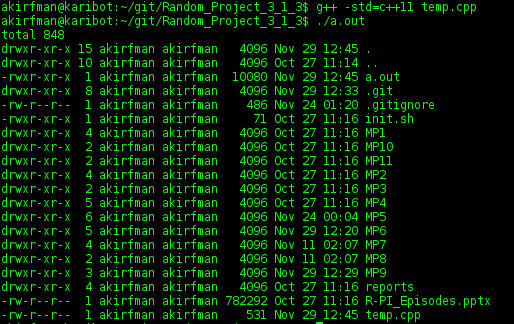
\includegraphics[scale=0.8]{e2_output.png}
    \end{center}

    \ \\
    When a UNIX/LINUX system starts up, two processes are initialized by the kernel.  The first, process 0, is known as the swapper.  As its name implies, it controls the scheduling of all processes on the system.  The second, process 1, is known as init.  Init is critical in the initialization of the system and starts many important routines (This includes the login shell).  Afterwards, all other new processes are created using fork and exec.  

    \ \\
    \textbf{fork()};
    
    \ \\
    When the operating system is initialized, three processes are created.  The first, known as the swapper (process id 0), serves as the scheduler for jobs on the system.  The second, known as init (process id 1), sets up many processes and services across the system.  After it performs its initial tasks, init becomes a looping call to wait() which reclaims the state of orphaned processes.  The third, known as the pagedaemon (process id 2), is responsible for memory management.  
    
    \ \\
    Other than these three processes started by the operating system, every other process in the system is brought to life through a call to the \code{fork()} system call.  A process calling fork is copied by the kernel.  At this point, the process that called fork is known as the parent, and the newly created process is known as the child since the parent process caused the child to be created.  The newly created process is essentially exactly the same as the child, even having the exact same variables and open files.  Fork is unique in that it is called once by the parent process and returns twice (to the parent and child separately).  To the parent, fork returns the process id (PID) of the newly created child.  To the child, fork returns 0.  If the call fails entirely, -1 is returned to the parent, and no child is created.  For more information about fork, see its manpage by calling \code{man 2 fork}.  
    
    \ \\
    Copying the entire context of a process could take quite a long time, especially if the parent process contains a large amount of data.  Instead, modern kernels perform an action called copy-on-write.  When the fork call returns, both processes point to the same regions in memory.  As soon as either process wants to write data anywhere in the address space, the kernel creates a new page in memory for that process.  Therefore, both processes use essentially all of the same memory regions initially, and they slowly diverge as time progresses.  
    
    \ \\
    A pseudocode description of the actual fork algorithm is provided below (Bach).  
    \vspace{5mm}

\begin{lstlisting}[frame=single]
(*@algorithm fork@*)
(*@input:@*)  (*@none@*)
(*@output: to parent proces, child PID number@*)
        (*@to child process. 0@*)
{
    (*@check for available kernel resources;@*)
    (*@get free proc table slot and unique PID number;@*)
    (*@check that user not running too many processes;@*)
    (*@mark child state as "being created";@*)
    (*@copy data from parent proc tabgle slot to new child slot;@*)
    (*@increment counts on current directory inode and changed root (if applicable);@*)
    (*@increment open file counts in file table;@*)
    (*@make copy of parent context (PCB, text, data, stack) in memory);@*)
    (*@push dummy system level context layer onto child system level context;@*)
        (*@dummy context contains data allowing child process to recognize@*)
        (*@itself, and start running from here when scheduled@*)
    (*@if(executing process is parent process)@*)
    {
        (*@change child state to "ready to run";@*)
        (*@return(child ID);@*)
    }
    (*@else@*)
    {
        (*@initialize PCB timing fields;@*)
        (*@return(0);@*)
    }
}
\end{lstlisting}
    
    \vspace{3mm}
    \ \\
    \textbf{The Six Exec Functions}
    
    \ \\
    After executing \code{fork()}, you are left with two identical processes.  This isn't usually particularly useful unless you specifically need two exact copies of a process.  Instead, UNIX provides a function, known as exec, which allows you to change a process's address space in order to run an entirely new program.  Running an exec command deletes the existing text, data, and stack segments of the existing process and replaces them with with those of a new program.  The algorithm for exec is presented below (Bach 218).  
    
\ \\
\begin{lstlisting}[frame=single]
(*@algorithm exec@*)
(*@input: @*)  (*@(1) file name@*)
        (*@ (2) parameter list@*)
        (*@ (3) environment variables list@*)
(*@output: none@*)
{
    (*@get file inode (algorithm namei);@*)
    (*@very file is executable and user has permission to execute;@*)
    (*@read file headers, check that it is a load module;@*)
    (*@copy exec parameters from old address space to system space;@*)
    (*@for(every region attached to process)@*)
    {
        (*@detach all old regions (algorithm detach);@*)
    }
    (*@for(every region specified in load module)@*)
    {
        (*@allocate new regions (algorithm allocreg);@*)
        (*@attach the regions (algorithm attachreg);@*)
        (*@load region into memory if appropriate (algorithm loadreg);@*)
    }
    (*@copy exec parameters into new user stack region;@*)
    (*@special processing for setuid programs, tracing;@*)
    (*@initialize user register save area for return to user mode;@*)
    (*@release inode of file (algorithm iput)@*)
}
\end{lstlisting}

    \ \\
    In UNIX systems, there is only one algorithm for exec, but the system call interface provides a total of six different variations of the exec function which differ only on how they handle input arguments.  This means that only one system call (usually \code{execve()}) is actually required to be implemented.  The other functions are stubs with perform necessary preparations and then eventually call execve.  Short function descriptions of each version are provided below (Setvens 207-209).  

    \begin{center}
        Example \#1: Exec Functions
    \end{center}
\begin{lstlisting}[frame=single]
#include<unistd.h>

1. int execl(const char *pathname, const char *arg0, ... (*@/* (char *) 0 */ @*));

2. int execv(const char *pathname, char *const argv[]);


(*@The following exec commands take an environment array (envp) in addition @*)
(*@to the other arguments.  This can be used to define a custom environment @*)
(*@for the process.  Otherwise, uses parent's environment.  @*)

3. int execle(const char *pathname, const char *arg0, ... (*@/* (char *) 0 */ @*), 
    char *const envp[]);

4. int execve(const char *pathname, char *const argv[], char *const envp[]);

(*@Exec commands ending in a p use the PATH environ variable in order to find@*)
(*@the executable file.  An error is thrown if the file is not in a directory@*)
(*@specified by PATH.  @*)

5. int execlp(const char* filename, const char *arg0, ... (*@/* (char *) 0 */ @*));

6. int execvp(const char *filename, char *const argv[]);

(*@All return -1 on error and do not return when successful@*)
\end{lstlisting}

    \begin{center}
        Figure \#4: Relationship of exec functions
    \end{center}
    \begin{center}
        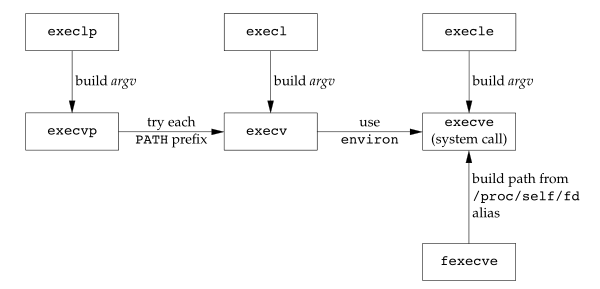
\includegraphics{relationship.png}
    \end{center}

\end{myindentpar}
    

\newpage
\noindent
{\large \underline{UNIX man Pages}:}

\begin{myindentpar}{5mm}

    One incredibly useful feature of UNIX operating systems that many new developers do not know about is the built in manual system.  Using the command 'man', you can access information about most aspects of the operating system from general commands all the way to system call APIs.  
    
    \ \\
    The structure of man pages in UNIX are organized into sections by number follows (Wikimedia Foundation):
    \begin{enumerate}
        \setlength\itemsep{-0.1em}
        
        \item General Commands
        \item System Calls
        \item Library Functions (Specifically, the C standard library)
        \item Special Files
        \item File Formats
        \item Games
        \item Miscellanea
        \item System Administration
        
    \end{enumerate}
    
    \ \\
    You may (or may not, that's fine too) find the following manual pages useful when creating this assignment.  Each one of these lines can be executed as a valid shell command to open a particular manual page.  Note, the number indicates the manual section that that function resides.  
    
    \begin{itemize}
        \setlength\itemsep{-0.1em}
    
        \item \code{man 3 exec}
        \item \code{man 2 fork}
        \item \code{man 2 chdir}
        \item \code{man 2 pipe}
        \item \code{man 2 dup}
        \item \code{man 2 wait}
     
    \end{itemize}

\end{myindentpar}

\newpage
\noindent
{\large \underline{Bibliography}:}

\ \\
{[} 1 {]} \hspace{1.2mm} Bovet, Daniel Pierce. \textit{Understanding the Linux Kernel: From I/O Ports to Process}
\hspace*{1cm} \textit{Management}. U.S.A: O'Reilly, 2003. Print.

\ \\
{[} 2 {]} \hspace{1.2mm} Glass, Graham. \textit{Linux for Programmers and Users}. Upper Saddle River, NJ: Pearson
\hspace*{1cm} Prentice Hall, 2006. Print.


\end{document}
